\documentclass[a4paper]{article}

\usepackage[portuguese]{babel}
\usepackage[utf8]{inputenc}
\usepackage[T1]{fontenc}

\newcommand{\documentTitle}{Genetic Algorithms - Brachistochrone Curve} %Macro definition
\newcommand{\documentAuthors}{João Rafael (2008111876, jprafael@student.dei.uc.pt) \and José Ribeiro (2008112181, jbaia@student.dei.uc.pt)} %Macro definition

\title{\documentTitle}
\author{\documentAuthors{}}

\usepackage{hyperref}
\hypersetup{
	pdftitle = \documentTitle
	,pdfauthor = \documentAuthors
	,pdfsubject = {Introduction to Artificial Inteligence Project \#2 Report}
	,pdfkeywords = {Artificial Inteligence Project} {Genetic Algorithms} {Brachistochrone Curve}
	,pdfborder = {0 0 0}
}

\usepackage{subfig}
\usepackage{amsmath}
\usepackage{wrapfig}
\usepackage{array}
\usepackage{anysize}
\usepackage{lscape}
\usepackage[pdftex]{graphicx}
\usepackage{longtable}
\usepackage{multirow}
\usepackage[table]{xcolor}

\marginsize{3.5cm}{3.5cm}{3cm}{3cm}

\makeatletter

\begin{document}
\renewcommand{\figurename}{Figure}
\maketitle
\cleardoublepage

\tableofcontents
\cleardoublepage

\setlength{\parindent}{1cm}
\setlength{\parskip}{0.3cm}

\section{Introduction}
\indent \indent Este projecto está inserido no âmbito da disciplina de Introdução à Inteligência Artificial,
mais concretamente no seguimento do primeiro projecto, uma vez que implementamos outro tipo de Agentes: Agentes Adaptativos.

Ao contrário dos agentes já estudados (Reactivos), estes baseiam-se fundamentalmente em conceitos da Biologia, nomeadamente a teoria da Selecção Natural de Darwin aplicada à Genética.
Estes agentes representam populações que, ao longo do tempo (iterações da aplicação), evoluem ao sofrer mutações e recombinações entre indivíduos (e os seus genes) e posterior selecção dos mais aptos.
Desta forma, pretende-se que a aptidão da população melhore, convergindo para o óptimo global.

\subsection{Brachistochrone curve}

\indent \indent O problema da curva braquistócrona é um clássico da disciplina de cálculo:

\emph{Tendo dois pontos distintos, A e B, o objectivo é conhecer a trajectória que minimiza o tempo que um ponto material demora a deslocar-se entre eles, quando sujeito apenas à força da gravidade (com atrito desprezável).}

\begin{figure}[ht]
	\centering
	\includegraphics[scale=0.5]{images/Brachistochrone.png}
	\caption{Curva Braquistócrona}
	\label{fig:brachistochrone}
\end{figure}

\indent Este problema apenas é válido quando se consideram pares de pontos com a altura de B inferior à de A, pois caso contrário o corpo não consegue efectuar o percurso.

Leibniz, L'Hospital, Newton, e os irmãos Bernoulli apresentaram soluções analíticas.
No entanto o estudo deste problema, segundo o paradigma de agentes adaptativos, é interessante pois permite calcular uma aproximação da curva
não necessitando de ferramentas matemáticas complexas.

\indent Para cada instância do problema, um indivíduo representa uma trajectória possível. Estes individuos são avaliados segundo uma
função de aptidão que mede o tempo correspondente: quanto menor, mais apto ele é considerado.

\indent De forma a definir o o formato da trajectória, cada indivíduo é caracterizado por um conjunto de genes. Estes representam os vários
factores que contribuem para a forma da trajectória, como por exemplo coordenadas, declives, curvaturas, etc. Assim, para alterar as características
de um determinado indivíduo (fenótipo) é necessário efectuar alterações ao seu conjunto genético (genótipo). Estas alterações podem se categorizar
fundamentalmente em dois tipos:

\begin{description}
	\item[Mutation] \hfill \\ 
		Alteração ou substituição de um gene por outro de origem primariamente estocástica.
	\item[Crossover] \hfill \\ 
		Aplicação de permutações no código genético de dois ou mais indivíduos, trocando a informação genética de um para outro.
\end{description}

\cleardoublepage
\section{Implementation}
\indent \indent Durante a implementação deste projecto foram surgindo abordagens alternativas,
introduzidas tanto por erros conceptuais, como por \emph{bugs}. Estas abordagens, apesar de não estarem de acordo com
o considerado comum na àrea de Inteligência Artificial, foram demonstrando capacidade de gerar soluções adequadas ao problema.
Assim, decidimos que seria interessante efectuar uma comparação entre os resultados obtidos segundo o método tradicional, e aquele a que apelidámos \emph{Rafael-Ribeiro}. 

\subsection{Representation}
\indent \indent À semelhança de outros problemas\footnote[1]{Aplicação do método do trapézio para o cálculo do integral de uma curva.}, a discretização do espaço contínuo em amostras
distintas facilita a computação numérica dos resultados. Desta forma escolhemos implementar duas formas de representação:

\begin{description}
	\item[Fixed] \hfill \\ 
		Onde a curva é aproximada por um conjunto sucessivo de segmentos de recta, definidos por pares de pontos equidistantes.
	\item[Dynamic] \hfill \\ 
		Uma representação da mesma natureza que a anterior, apenas retirando a restrição da distância entre pontos.
\end{description}

\indent Estas duas representações foram escolhidas por serem compactas, i.e.: para cada gene apenas é necessário guardar a informação das suas coordenadas.
Note-se que no caso da representação fixa a absissa é conhecida \emph{a priori}, reduzindo assim o espaço de procura exponencialmente (em relação à dinâmica).

\indent Para além destas duas representações considerámos ainda uma terceira:

\begin{description}
	\item[NURBS] \hfill \\ 
		A curva aproximada é definida à custa dos pontos de controlo de uma NURBS\footnote[2]{Non-uniform rational basis spline.}. 
		\begin{figure}[ht]
			\centering
			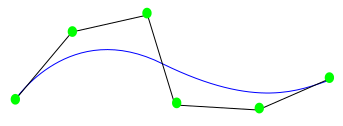
\includegraphics[scale=0.50]{images/NURBstatic.png}
			\caption{Exemplo de uma NURBS}
			\label{fig:nurbs}
		\end{figure}
\end{description}

\indent A principal vantagem desta representação é o facto de se basear em polinómios de grau superior a um, o que permite aproximar a curva desejada
com igual rigor utilizando um conjunto de pontos inferior. Desta forma o espaço de procura é mais reduzido, pelo que a convergência do algoritmo
seria esperadamente mais rápida.

\indent No entanto esta representação também apresenta os seus problemas: a avaliação da aptidão de um indivíduo depende do cálculo da derivada
desta curva, o que representa por si só um problema merecedor de uma análise profunda. 

\cleardoublepage
\subsection{Mutation Operators}
\indent \indent Um dos principais factores que contribuem para a performance de um algoritmo genético é a diversidade genética presente na população.
Desta forma, desenvolver os operadores de mutação adequados para cada problema torna-se uma tarefa crucial.
Estes actuam ao nível de cada gene e são portanto distintos para cada representação. 

\subsubsection{Fixed Representation}
\indent \indent Nesta representação o único parâmetro que se altera são as coordenadas \emph{yy} de cada gene.
Para sortear o novo valor a atribuir foi utilizada uma distribuição gaussiana (ao invés de uniforme), com o intuito 
de garantir que a evolução progenitor-filho é efectuada de forma gradual (i.e.: que o filho preserva algumas características dos
seus antecessores).

\subsubsection{Dynamic Representation}
\indent \indent Ao contrário da representação anterior, o operador de mutação para a representação dinâmica necessíta de considerar
tanto as coordenadas \emph{yy} como as \emph{xx}. Pelas razões já enunciadas, a distribuição utilizada foi novamente a gaussiana.
No entanto, uma vez que esta permite alterar a posição relativa dos pontos, é necessário efectuar um ordenamento posterior.

\indent Como estes operadores se aplicam a genes individualmente, é necessário escolher quais genes sofrem mutação.
O operador tradicional aplica uma igual probabilidade a cada gene. No entanto, segundo o paradigma biológico,
a probabilidade de erros consecutivos é mais elevada (pois a anomalia que levou à criação do primeiro erro pode ainda verificar-se).
Como achamos que esta abordagem poderia ser vantajosa para o problema em questão, decidimos implementar dois modelos de mutações adicionais:

\begin{description}
	\item[Burst] \hfill \\ 
		Onde indicamos a probabilidade de um gene ser mutado após o seu antecessor também o ser.

	\item[Range] \hfill \\ 
		Onde por cada indivíduo é apenas selecionado uma secção de genes que sofre mutação.
		Este tipo de mutação é apenas aplicado para o tipo de selecção \emph{Rafael-Ribeiro}.
\end{description}
 
\cleardoublepage
\subsection{Crossover Operator}
\indent \indent O operador de recombinação distingue-se do operador de mutação na forma como tem impacto no material genético da população.
Enquanto que o operador de mutação actua sobre um único indivíduo (o que introduz novo material genético na população),
o operador de recombinação reorganiza o material genético já existente, conseguindo propagar as características entre indivíduos.
Este operador aliado a um tipo de selecção adequado (ver \ref{subsec:selection}) permite uma melhor convergência
do algoritmo.

\subsubsection{Fixed Representation}
\indent \indent Nesta representação, após o sorteio do número de pontos de recombinação (que não excede um máximo estabelecido) o operador
sorteia as coordenadas em que tais pontos de recombinação se vão aplicar, efectuando as trocas correspondentes.

\subsubsection{Dynamic Representation}
\indent \indent Dada a natureza da representação, as coordenadas sorteadas para pontos de recombinação não \emph{têm} que necessariamente existir no indivíduo.
Como tal, as coordenadas entre cada ponto de recombinação são trocadas entre si, independentemente deste processo recombinar mais ou menos genes.
Após este processo, é aplicado sobre os indivíduos com maior número de pontos (que o valor pré-definido) o operador de remoção de genes; sobre os indivíduos com menor
número de pontos é aplicado o operador de interpolação de pontos, por forma a perfazer o total de pontos do indivíduo.

\cleardoublepage
\subsection{Selection}
\label{subsec:selection}
\indent \indent Após a criação de novos descendentes é necessário efectuar uma redução no número de indivíduos.
Desta forma é possível garantir que o tamanho da população continua computacionalmente tratável e que o algoritmo convirja tendencialmente para o óptimo global.

\indent De notar que o elitismo é usualmente utilizado (excepto na selecção Rafael-Ribeiro) simultaneamente com selecção por roleta ou torneio.

\begin{description}
	\item[Elitism] \hfill \\
		Abordagem gananciosa que seleciona os melhores indivíduos da população como descendetes.

	\item[Roulette] \hfill \\
		Os indivíduos são selecionados de forma aleatória, dando maior probabilidade aos indivíduos com maior fitness.
		Para garantir esta propriedade a função de probabilidade para um indivíduo $i$ é:

		\[
			p_{i} = \frac{f_{i}}{\sum\limits_{j \in \text{Pop.}} f_{j}} \quad \text{onde} \quad f_i = \frac{1}{T_{i}} \quad (T_{i} \leftarrow \text{Tempo correspondente ao indivíduo } i)
		\]

		Neste algoritmo o mesmo elemento pode ser escolhido várias vezes,
		simulando a capacidade de um ser mais apto se conseguir reproduzir com maior frequência.

	\item[Tournament] \hfill \\ 
		Para este tipo de selecção são escolhidos aleatoriamente N indivíduos, dos quais apenas o mais apto é escolhido.
		Após esta selecção todos os elementos participantes no torneio são devolvidos à população.

	\item[Rafael-Ribeiro] \hfill \\
		Nesta abordagem implementa-se em conjunto a selecção por elitismo e por torneio, mas ao contrário da abordagem tradicional
		esta é aplicada não só para selecionar os progenitores, mas também para selecionar que indivíduos da população inteira (pais e filhos)
		sobrevivem para a próxima iteração. Do ponto de vista que apenas alguns indivíduos são alterados, este tipo de selecção pode ser considerada \emph{Steady-State}.

\end{description}

\indent \indent 


\cleardoublepage

\subsection{...}
\indent \indent ...

\subsection{...}
\indent \indent ...

\subsubsection{...}
\indent \indent ...

\subsubsection{...}
\indent \indent ...

...

\cleardoublepage
\subsection{...}
\indent \indent ...

...

\subsection{...}
\indent \indent ...

...

\subsection{...}
\indent \indent ...

\cleardoublepage

\section{Experiments}
\indent \indent ...

\cleardoublepage

\subsection{...}
\indent \indent ...

\cleardoublepage

\section{Validation}
\indent \indent Para validar o comportamento do Agente, cada combinação de parâmetros foi executada 30 vezes com seeds diferentes;
tal garante que a natureza estocástica do algoritmo fica evidenciada ao garantir que os testes são, de facto, diferentes.

Após a conclusão dos testes, foi calculado o desvio-padrão entre as 30 simulações,
para averiguar se os resultados obtidos não representavam apenas um caso de sorte.

Tal como se pode verificar na última coluna da tabela de resultados (Secção \ref{tab:results}), o desvio-padrão entre as 30 simulações para cada combinação de parâmetros
é bastante reduzido, o que comprova a sua consistência e robustez.

\cleardoublepage

\subsection{...}
\indent \indent ...

\cleardoublepage

\section{Result Analysis}
\indent \indent ...

\cleardoublepage
\subsection{Representation}
\begin{center}
	\begin{center}
	\begin{tabular}{|c|c|c|c|c|}
		\hline
		\multirow{3}{*}{Iterations}	&	\multicolumn{4}{c|}{Best fitness by representation}	\\
										\cline{2-5}
									&	\multicolumn{2}{c|}{Points set 1}	& \multicolumn{2}{c|}{Points set 2} \\
										\cline{2-5}
									&	Even			&	Dynamic			&	Even			&	Dynamic		\\
		\hline								
		20							& 1.2943594 \cellcolor[gray]{0.9}		& 1.4232276			& 1.6813473 \cellcolor[gray]{0.9}		& 1.7981805		\\
		\hline
		100							& 1.2334137 \cellcolor[gray]{0.9}		& 1.2447508 		& 1.4464484 \cellcolor[gray]{0.9}		& 1.5103336		\\
		\hline
		1000						& 1.2221068 		& 1.2149932 \cellcolor[gray]{0.9}		& 1.4182575 		& 1.4090841	\cellcolor[gray]{0.9}	\\
		\hline
		2000						& 1.2216529 		& 1.2140057 \cellcolor[gray]{0.9}		& 1.4166809 		& 1.4074098	\cellcolor[gray]{0.9}	\\
		\hline
	\end{tabular}
	\label{tab:selection_type}
\end{center}

\begin{center}
	\begin{tabular}{|c|c|c|c|c|}
		\hline
		\multirow{3}{*}{Iterations}	&	\multicolumn{4}{c|}{Bests' average fitness by representation}	\\
										\cline{2-5}
									&	\multicolumn{2}{c|}{Points set 1}	& \multicolumn{2}{c|}{Points set 2} \\
										\cline{2-5}
									&	Even			&	Dynamic			&	Even			&	Dynamic		\\
	\hline								
	20								&	2.0605766  \cellcolor[gray]{0.9}		&	2.2695527		&	2.2065896  \cellcolor[gray]{0.9}		&	2.2270115	\\
	\hline
	100								&	1.5433335  \cellcolor[gray]{0.9}		&	1.7756616		&	1.8700758  \cellcolor[gray]{0.9}		&	1.8953272	\\
	\hline
	1000 							&	1.3103644  \cellcolor[gray]{0.9}		&	1.4003977		&	1.6023816  \cellcolor[gray]{0.9}		&	1.6161404	\\
	\hline
	2000							&	1.2970950  \cellcolor[gray]{0.9}		&	1.3512935		&	1.5659681  \cellcolor[gray]{0.9}		&	1.5721760	\\
	\hline
	\end{tabular}
	\label{tab:selection_type}
\end{center}

\end{center}

\subsection{Selection}
\begin{center}
	\begin{center}
	\begin{tabular}{|c|c|c|c|c|c|c|}
		\hline
		\multirow{3}{*}{Iterations}	&	\multicolumn{6}{c|}{Points set 1}	\\
										\cline{2-7}
									&	\multicolumn{3}{c|}{Even}	& \multicolumn{3}{c|}{Dynamic} \\
										\cline{2-7}
									&	Tournament		&	Roulette		&	Rafael-Ribeiro	&	Tournament		&	Roulette		&	Rafael-Ribeiro		\\
		\hline
		20							&	1.3035679		& 	1.2943594		&	1.4051295		&	1.4306861		&	1.4232276		&	1.5133809			\\
		\hline
		100							&	1.2339894		&	1.2334137		&	1.2337409		&	1.2447508		&	1.2462901		&	1.2587349			\\
		\hline
		1000						&	1.2260637		&	1.2257382		&	1.2221068		&	1.2152843		&	1.2149932		&	1.2155451			\\
		\hline
		2000						&	1.2249858		&	1.2248156		&	1.2216529		&	1.2140487		&	1.2140057		&	1.2143467			\\
		\hline
	\end{tabular}
	\label{tab:selection_type_1}
\end{center}

\begin{center}
	\begin{tabular}{|c|c|c|c|c|c|c|}
		\hline
		\multirow{3}{*}{Iterations}	&	\multicolumn{6}{c|}{Points set 2}	\\
										\cline{2-7}
									&	\multicolumn{3}{c|}{Even}	& \multicolumn{3}{c|}{Dynamic} \\
										\cline{2-7}
									&	Tournament		&	Roulette		&	Rafael-Ribeiro	&	Tournament		&	Roulette		&	Rafael-Ribeiro		\\
		\hline
		20							&	1.6924473		&	1.6813473		&	1.8522521		&	1.7981805		&	1.8119160		&	1.8816109			\\
		\hline
		100							&	1.4471459		&	1.4464484		&	1.5623404		&	1.5140132		&	1.5103336		&	1.5691733			\\
		\hline
		1000						&	1.4208745		&	1.4209846		&	1.4182575		&	1.4094479		&	1.4093918		&	1.4090841			\\
		\hline	
		2000						&	1.4195882		&	1.4198324		&	1.4166809		&	1.4074098		&	1.4074232		&	1.4074481			\\
		\hline
	\end{tabular}
	\label{tab:selection_type_2}
\end{center}

\end{center}

\cleardoublepage
\subsection{Crossover}
%TODO

\subsection{...}
\indent \indent ...

\cleardoublepage
\section{Conclusion}
\indent \indent ...

\cleardoublepage

\subsection{...}
\indent \indent ...

\cleardoublepage
\section{Anexos}

\eject \pdfpagewidth=594.0mm \pdfpageheight=420.0mm

\subsection{Tabela de Resultados}
\begin{center}
	\input{tables/results}
\end{center}

\end{document}
